\documentclass[12pt]{article}

\usepackage[spanish]{babel}
\selectlanguage{spanish}
\usepackage[utf8]{inputenc}
\usepackage{vmargin}
\usepackage{graphicx}
\setmargins{2.5cm}{1.5cm}{16.5cm}{23.42cm}{0pt}{1cm}{0pt}{2cm}

\title{Polinomios de Taylor en Gnuplot}
\author{Martín Alejandro Paredes Sosa}
\date{Marzo 2015}
\graphicspath{{IMG/}}

\begin{document}
\maketitle
\section{Polinomio de Taylor}
En cálculo, el teorema de Taylor, recibe su nombre del matemático británico Brook Taylor, quien lo enunció con mayor generalidad en 1712, aunque previamente James Gregory lo había descubierto en 1671. Este teorema permite obtener aproximaciones polinómicas de una función en un entorno de cierto punto en que la función sea diferenciable. Además el teorema permite acotar el error obtenido mediante dicha estimación. \\ \\
	Este teorema permite aproximar una función derivable en el entorno reducido alrededor de un punto $x_0 \in (a, b)$ mediante un polinomio cuyos coeficientes dependen de las derivadas de la función en ese punto. Más formalmente, si $ n \geq 0 $ es un entero y $ f $ una función que es derivable n veces en el intervalo cerrado $[a,x]$ y  n+1 veces en el intervalo abierto $(a,x)$, entonces se cumple que:

	$$ P_T(x)= f(x_o)+f'(x_o)(x-x_o)+ {f^{(2)}(x_o)\over 2!}(x-x_o)^2+\cdots+{f^{(n)}(x_o)\over n!}(x-x_o)^n+E_n $$
Donde:
	$$ E_n={f^{(n+1)}(c)\over (n+1)	!}(x-x_o)^{n+1} $$
De manera compacta:
	$$ P_T(x)=\sum^n_{k=0} {f^{(k)}(x_o)\over k!}(x-x_o)^k$$ 


\section{Aproximaciones con polinomio de Taylor}
La siguiente practica consistió en estimar polinomios de Taylor para la función dada. Se tomaron diversas funciones y se estimó el polinomio de grado $n$ con el programa wxMaxima. Luego se graficaron los polinomios encontrados con herramientas de gnuplot en Maxima.
\pagebreak
\subsection{Aproximación de $Sin(x)$}
Codigo Maxima
\begin{verbatim}
f(x):= sin(x);
t(x):=taylor(f(x), x, 0, 1);
t2(x):=taylor(f(x), x, 0, 3);
t3(x):=taylor(f(x), x, 0, 5);
t4(x):=taylor(f(x), x, 0, 7);

plot2d ([f(x),t(x),t2(x),t3(x),t4(x)],[x, -%pi, %pi], [y, -1.55, 1.55],
[legend,false], [xlabel,"x"], [ylabel,"Sin(x)"],[axes, solid], [box, false],
[color, red, green, blue, orange, gray],[title,"Sin(x)"],[label,
["y=P1(x)",1.4,1.27],["y=P5(x)",2.65,0.7],["y=sin(x)",2.75,0.45],
["y=P7(x)",2.65, 0.05],["y=P3(x)",2.35,-1],["y",-0.4,1.5],["x", 3.1,-0.15]]);

tex(f(x));
tex(t(x));
tex(t2(x));
tex(t3(x));
tex(t4(x));
\end{verbatim}
Los resultados que se obtuvieron fueron:
\begin{itemize}
\item{$P_1=x+\cdots $}
\item{$P_3=x-{{x^3}\over{6}}+\cdots $}
\item{$P_5=x-{{x^3}\over{6}}+{{x^5}\over{120}}+\cdots$}
\item{$P_7=x-{{x^3}\over{6}}+{{x^5}\over{120}}-{{x^7}\over{5040}}+\cdots $}
\end{itemize}
Por último un gráfico de las funciones:
\begin{center}
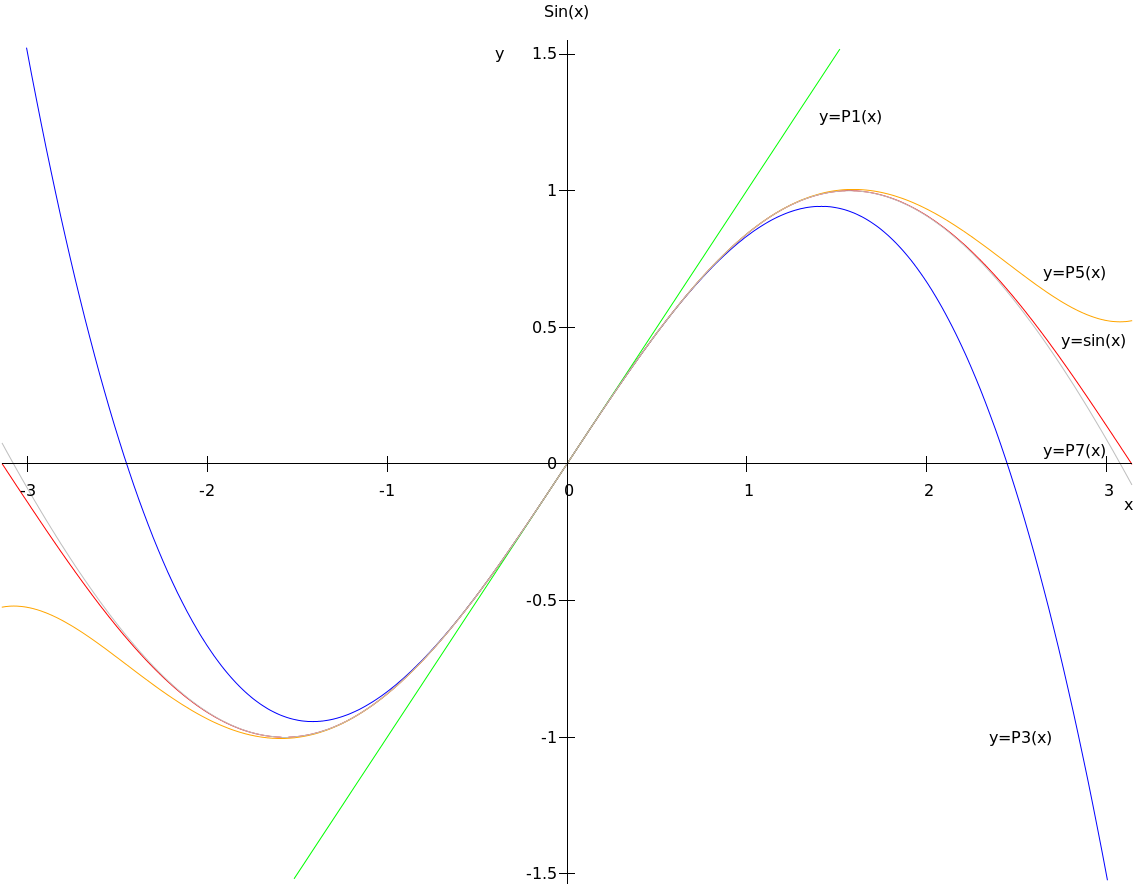
\includegraphics[width=10cm]{TaylorSin(x)}
\end{center}
\pagebreak

\subsection{Aproximación de $log(1+x)$}
Codigo Maxima
\begin{verbatim}
f(x):= log(1+x);
t(x):=taylor(f(x), x, 0, 4); t2(x):=taylor(f(x), x, 0, 7);
t3(x):=taylor(f(x), x, 0, 11); t4(x):=taylor(f(x), x, 0, 16);

plot2d ([t(x),t2(x),t3(x),t4(x),f(x)], [x, -1.5, 1.5], [y, -4, 2],
[legend,"T4(x)","T7(x)","T11(x)","T16(x)","Log(1+x)"] ,
[xlabel,"x"], [ylabel,"Log(1+x)"],[color, red, green, blue, cyan, orange],
 grid2d, [yx_ratio,1.3],[xtics,0.5],[ytics,0.5],
[gnuplot_preamble,"set key left "]);

tex(f(x)); tex(t(x)); tex(t2(x)); tex(t3(x)); tex(t4(x));
\end{verbatim}
Los resultados que se obtuvieron fueron:
\begin{itemize}
\item{$P_4=x-{{x^2}\over{2}}+{{x^3}\over{3}}-{{x^4}\over{4}}+\cdots $}
\item{$P_7=x-{{x^2}\over{2}}+{{x^3}\over{3}}-{{x^4}\over{4}}+{{x^5}\over{5}}-{{x^6}\over{6}}+{{x^7}\over{7}}+\cdots $}
\item{$P_{11}=x-{{x^2}\over{2}}+{{x^3}\over{3}}-{{x^4}\over{4}}+{{x^5}\over{5}}-{{x^6}\over{6}}+{{x^7}\over{7}}-{{x^8}\over{8}}+{{x^9}\over{9}}-{{x^{10}}\over{10}}+{{x^{11}}\over{11}}+\cdots$}
\item{$P_{16}=x-{{x^2}\over{2}}+{{x^3}\over{3}}-{{x^4}\over{4}}+{{x^5}\over{5}}-{{x^6}\over{6}}+{{x^7}\over{7}}-{{x^8}\over{8}}+{{x^9}\over{9}}-{{x ^{10}}\over{10}}+{{x^{11}}\over{11}}-{{x^{12}}\over{12}}+{{x^{13}}\over{13}}-{{x^{14}}\over{14}}+{{x^{15}}\over{15}}-{{x^{16}}\over{16}}+\cdots $}
\end{itemize}
Por último un gráfico de las funciones:
\begin{center}
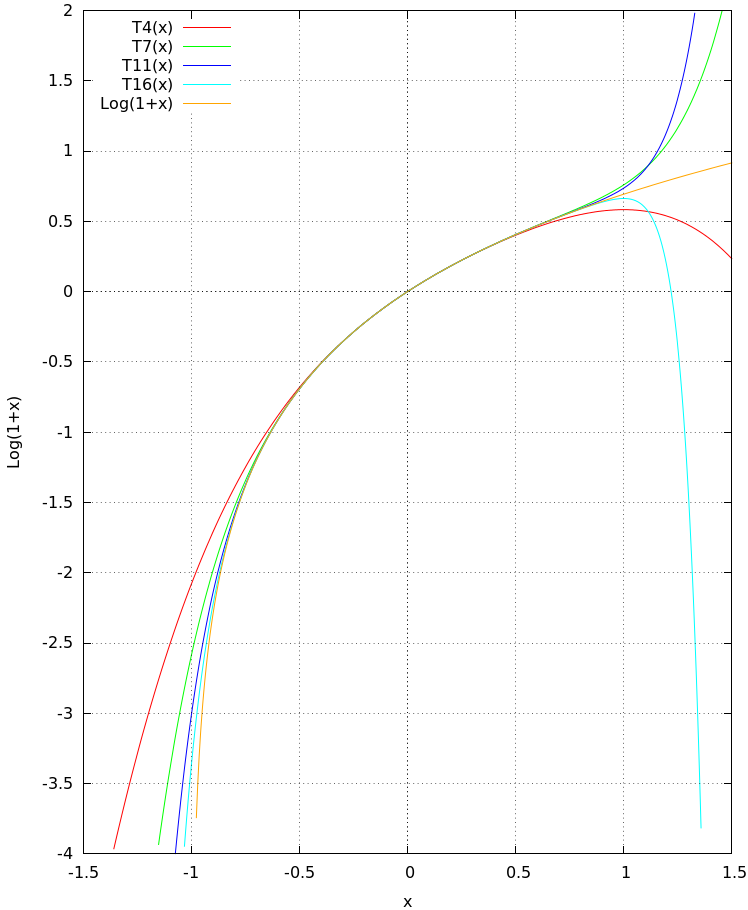
\includegraphics[height=10cm]{TaylorLog(1+x)}
\end{center}
\pagebreak

\subsection{Aproximación de $log(cos(x))$}
Codigo Maxima
\begin{verbatim}
f(x):= log(cos(x));
t(x):=taylor(f(x), x, 0, 1);
t2(x):=taylor(f(x), x, 0, 3);
t3(x):=taylor(f(x), x, 0, 5);
t4(x):=taylor(f(x), x, 0, 7);

plot2d ([f(x),t(x),t2(x),t3(x),t4(x)], [x, -%pi/2, %pi/2], [y, -1, .2],
[legend, "Log(Cos(x))","P1(x)","P3(x)","P5(x)","P7(x)"] ,
[xlabel,"x"], [ylabel,"Log(Cos(x))"]);

tex(f(x));
tex(t(x));
tex(t2(x));
tex(t3(x));
tex(t4(x));
\end{verbatim}
Los resultados que se obtuvieron fueron:
\begin{itemize}
\item{$P_1= 0+\cdots $}
\item{$P_3= {-{x^2}\over{2}}+\cdots  $}
\item{$P_5= {-{x^2}\over{2}}-{{x^4}\over{12}}+\cdots $}
\item{$P_7= {-{x^2}\over{2}}-{{x^4}\over{12}}-{{x^6}\over{45}}+\cdots  $}
\end{itemize}
Por último un gráfico de las funciones:
\begin{center}
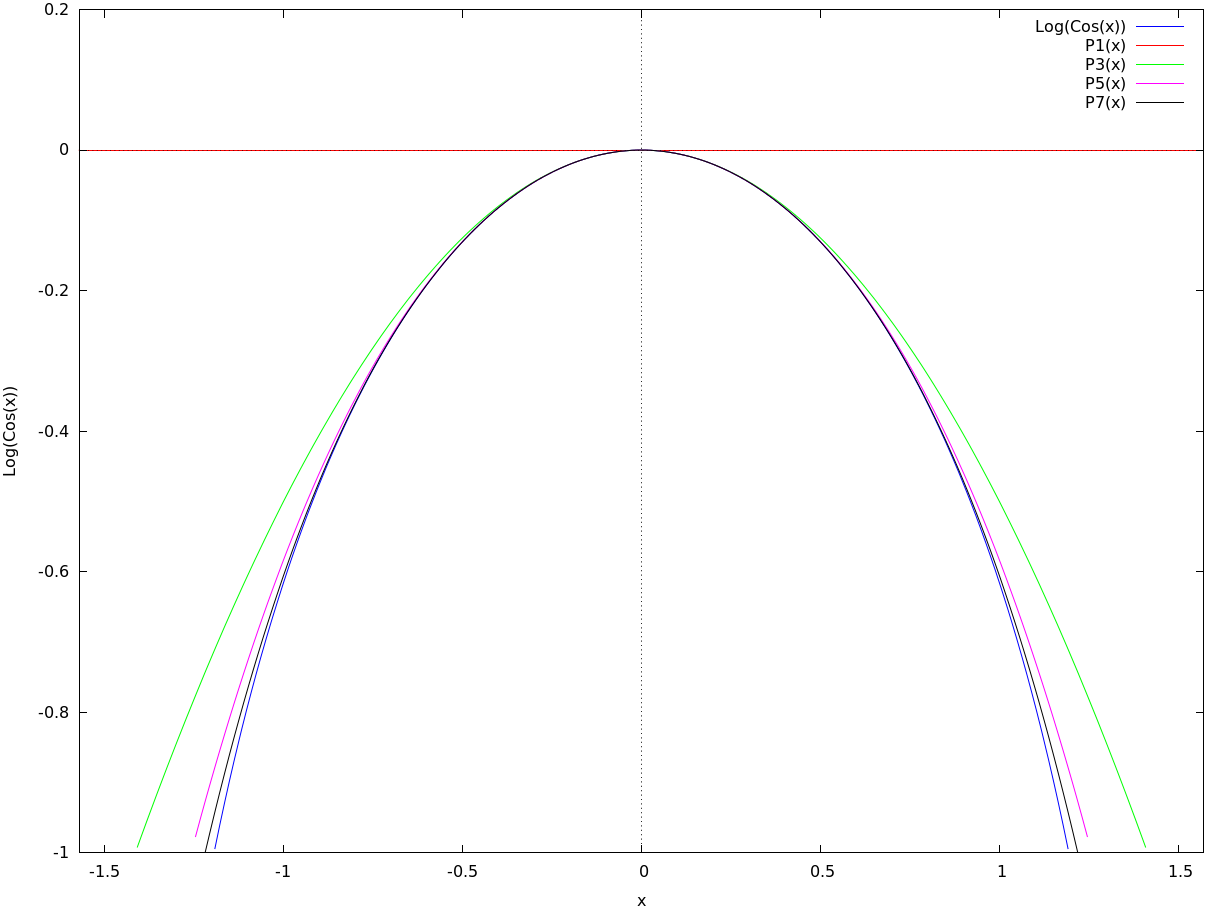
\includegraphics[width=12cm]{TaylorLog(cos(x))}
\end{center}
\pagebreak

\subsection{Aproximación de $ e^x \over cos(x)$}
Codigo Maxima
\begin{verbatim}
f(x):= exp(x)/cos(x);
t(x):=taylor(f(x), x, 0, 1);
t2(x):=taylor(f(x), x, 0, 3);
t3(x):=taylor(f(x), x, 0, 5);
t4(x):=taylor(f(x), x, 0, 7);

plot2d ([f(x),t(x),t2(x),t3(x),t4(x)], [x, -%pi, %pi], [y, -2, 2],
[legend, "Exp(x)/Cos(x)","P1(x)","P3(x)","P5(x)","P7(x)"] ,
[xlabel,"x"], [ylabel,"Exp(x)/Cos(x)"] );

tex(f(x));
tex(t(x));
tex(t2(x));
tex(t3(x));
tex(t4(x));
\end{verbatim}
Los resultados que se obtuvieron fueron:
\begin{itemize}
\item{$P_1= 1+x+\cdots $}
\item{$P_3= 1+x+x^2+{{2\,x^3}\over{3}}+\cdots  $}
\item{$P_5= 1+x+x^2+{{2\,x^3}\over{3}}+{{x^4}\over{2}}+{{3\,x^5}\over{10}}+\cdots $}
\item{$P_7= 1+x+x^2+{{2\,x^3}\over{3}}+{{x^4}\over{2}}+{{3\,x^5}\over{10}}+{{19\,x^6}\over{90}}+{{13\,x^7}\over{105}}+\cdots $}
\end{itemize}
Por último un gráfico de las funciones:
\begin{center}
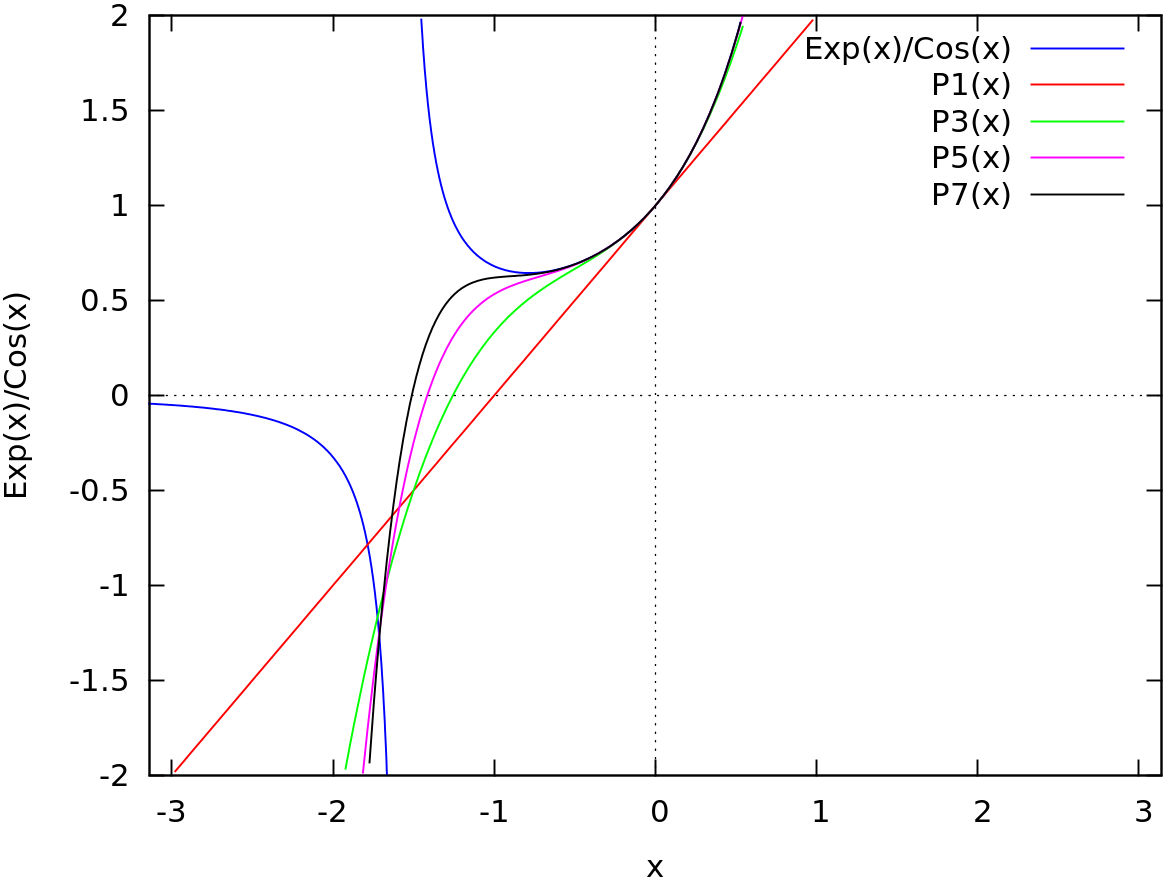
\includegraphics[width=12cm]{TaylorExp(x)Cos(x)}
\end{center}
\pagebreak
\subsection{Aproximación de $e^x(x+1)$}
Codigo Maxima
\begin{verbatim}
f(x):=(1+x)*exp(x);
t(x):=taylor(f(x), x, 0, 1);
t2(x):=taylor(f(x), x, 0, 3);
t3(x):=taylor(f(x), x, 0, 5);
t4(x):=taylor(f(x), x, 0, 7);

plot2d ([f(x),t(x),t2(x),t3(x),t4(x)], [x, -%pi, %pi], [y, -2, 2],
[legend, "(1+x)*Exp(x)","P1(x)","P3(x)","P5(x)","P7(x)"] ,
[xlabel,"x"], [ylabel,"(1+x)*Exp(x)"] );

tex(f(x));
tex(t(x));
tex(t2(x));
tex(t3(x));
tex(t4(x));
\end{verbatim}
Los resultados que se obtuvieron fueron:
\begin{itemize}
\item{$P_1= 1+2\,x+\cdots $}
\item{$P_3= 1+2\,x+{{3\,x^2}\over{2}}+{{2\,x^3}\over{3}}+\cdots $}
\item{$P_5= 1+2\,x+{{3\,x^2}\over{2}}+{{2\,x^3}\over{3}}+{{5\,x^4}\over{24}}+{{x^5}\over{20}}+\cdots $}
\item{$P_7= 1+2\,x+{{3\,x^2}\over{2}}+{{2\,x^3}\over{3}}+{{5\,x^4}\over{24}}+{{x^5}\over{20}}+{{7\,x^6}\over{720}}+{{x^7}\over{630}}+\cdots $}
\end{itemize}
Por último un gráfico de las funciones:
\begin{center}
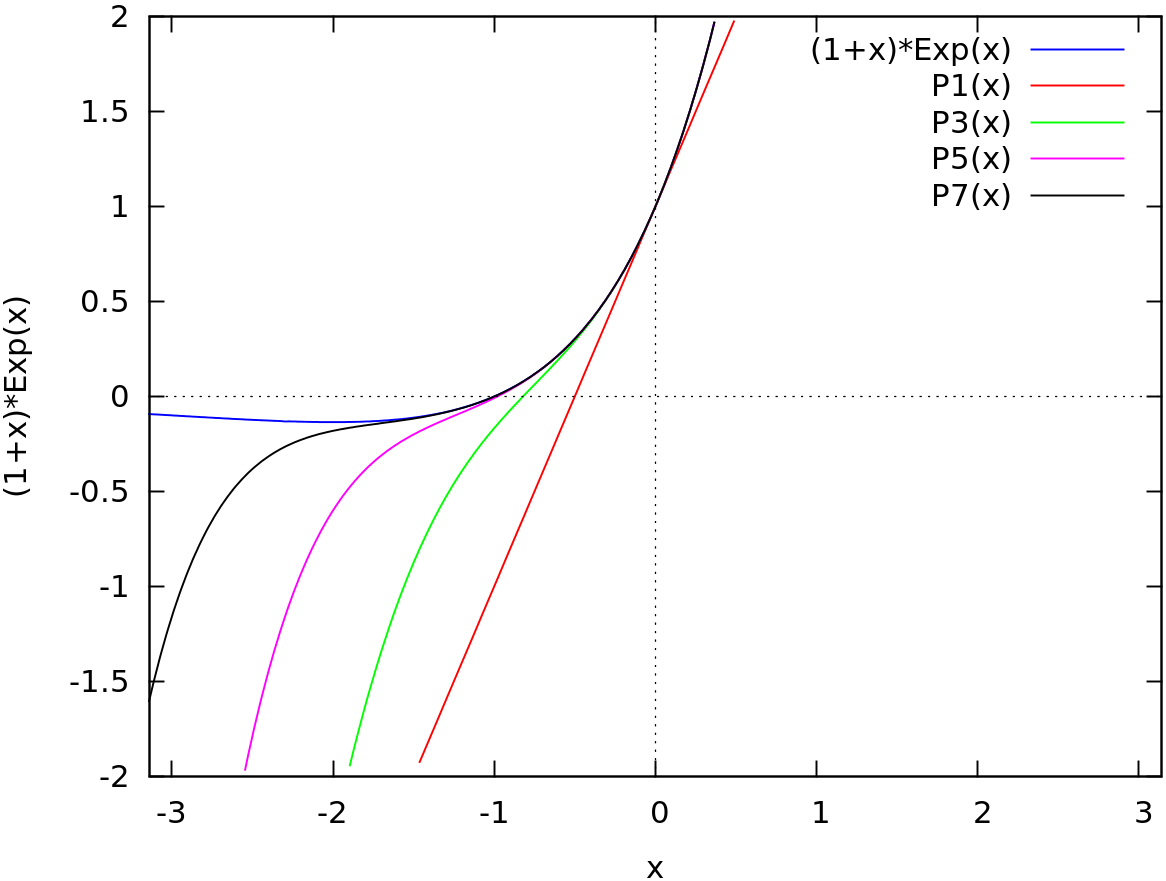
\includegraphics[width=12cm]{Taylor(1+x)Exp(x)}
\end{center}


\end{document}
